%%*************************************************************************
%% Helga Ingimundardottir, hei2@hi.is
%% LaTeX source code for ISDA 2011 paper #1569474013
%%   Sampling Strategies for Ordinal Regression in 
%%   Surrogate Assisted Evolutionary Optimization
%%
%% File list of work: isda2011.tex, isda2011.bib, isda2011.ps, isda2011.pdf, 
%% and figures figs/***.eps
%%   where *** are: anova, schema, rosen_meanFitness_funcEval, 
%%   rosen_intmEvals_gen, sphere_meanFitness_funcEval, sphere_intmEvals_gen
%%                    
%%*************************************************************************
%% NOTE: ps2pdf -dEmbedAllFonts=true -dSubsetFonts=true -dEPSCrop=true -dPDFSETTINGS=/prepress isda2011_hei2.ps

%\documentclass[10pt, conference, compsocconf]{IEEEtran} 
\documentclass[10pt, conference]{IEEEtran} % so paper is more compact
% Add the compsocconf option for Computer Society conferences.
%
% If IEEEtran.cls has not been installed into the LaTeX system files,
% manually specify the path to it like:
% \documentclass[conference]{../sty/IEEEtran}

% Some very useful LaTeX packages include:
% (uncomment the ones you want to load)

% *** MISC UTILITY PACKAGES ***
%
%\usepackage{ifpdf}
% Heiko Oberdiek's ifpdf.sty is very useful if you need conditional
% compilation based on whether the output is pdf or dvi.
% usage:
% \ifpdf
%   % pdf code
% \else
%   % dvi code
% \fi
% The latest version of ifpdf.sty can be obtained from:
% http://www.ctan.org/tex-archive/macros/latex/contrib/oberdiek/
% Also, note that IEEEtran.cls V1.7 and later provides a builtin
% \ifCLASSINFOpdf conditional that works the same way.
% When switching from latex to pdflatex and vice-versa, the compiler may
% have to be run twice to clear warning/error messages.






% *** CITATION PACKAGES ***
%
\usepackage{cite}
% cite.sty was written by Donald Arseneau
% V1.6 and later of IEEEtran pre-defines the format of the cite.sty package
% \cite{} output to follow that of IEEE. Loading the cite package will
% result in citation numbers being automatically sorted and properly
% "compressed/ranged". e.g., [1], [9], [2], [7], [5], [6] without using
% cite.sty will become [1], [2], [5]--[7], [9] using cite.sty. cite.sty's
% \cite will automatically add leading space, if needed. Use cite.sty's
% noadjust option (cite.sty V3.8 and later) if you want to turn this off.
% cite.sty is already installed on most LaTeX systems. Be sure and use
% version 4.0 (2003-05-27) and later if using hyperref.sty. cite.sty does
% not currently provide for hyperlinked citations.
% The latest version can be obtained at:
% http://www.ctan.org/tex-archive/macros/latex/contrib/cite/
% The documentation is contained in the cite.sty file itself.






% *** GRAPHICS RELATED PACKAGES ***
%
\ifCLASSINFOpdf
  \usepackage[pdftex]{graphicx}
  % declare the path(s) where your graphic files are
  \graphicspath{{figs/}}
  % and their extensions so you won't have to specify these with
  % every instance of \includegraphics
  \DeclareGraphicsExtensions{.eps}
\else
  % or other class option (dvipsone, dvipdf, if not using dvips). graphicx
  % will default to the driver specified in the system graphics.cfg if no
  % driver is specified.
  \usepackage[dvips]{graphicx}
  % declare the path(s) where your graphic files are
  \graphicspath{{figs/}}
  % and their extensions so you won't have to specify these with
  % every instance of \includegraphics
  \DeclareGraphicsExtensions{.eps}
\fi
% graphicx was written by David Carlisle and Sebastian Rahtz. It is
% required if you want graphics, photos, etc. graphicx.sty is already
% installed on most LaTeX systems. The latest version and documentation can
% be obtained at: 
% http://www.ctan.org/tex-archive/macros/latex/required/graphics/
% Another good source of documentation is "Using Imported Graphics in
% LaTeX2e" by Keith Reckdahl which can be found as epslatex.ps or
% epslatex.pdf at: http://www.ctan.org/tex-archive/info/
%
% latex, and pdflatex in dvi mode, support graphics in encapsulated
% postscript (.eps) format. pdflatex in pdf mode supports graphics
% in .pdf, .jpeg, .png and .mps (metapost) formats. Users should ensure
% that all non-photo figures use a vector format (.eps, .pdf, .mps) and
% not a bitmapped formats (.jpeg, .png). IEEE frowns on bitmapped formats
% which can result in "jaggedy"/blurry rendering of lines and letters as
% well as large increases in file sizes.
%
% You can find documentation about the pdfTeX application at:
% http://www.tug.org/applications/pdftex





% *** MATH PACKAGES ***
%
\usepackage{latexsym}
\usepackage[cmex10]{amsmath}\usepackage{amssymb}
% A popular package from the American Mathematical Society that provides
% many useful and powerful commands for dealing with mathematics. If using
% it, be sure to load this package with the cmex10 option to ensure that
% only type 1 fonts will utilized at all individual sizes. Without this option,
% it is possible that some math symbols, particularly those within
% footnotes, will be rendered in bitmap form which will result in a
% document that can not be IEEE Xplore compliant!
%
% Also, note that the amsmath package sets \interdisplaylinepenalty to 10000
% thus preventing page breaks from occurring within multiline equations. Use:
\interdisplaylinepenalty=2500
% after loading amsmath to restore such page breaks as IEEEtran.cls normally
% does. amsmath.sty is already installed on most LaTeX systems. The latest
% version and documentation can be obtained at:
% http://www.ctan.org/tex-archive/macros/latex/required/amslatex/math/

% Helga's math-shorthand
\newcommand{\inner}[2]{\big<{#1}\cdot{#2}\big>}
\renewcommand{\vec}[1]{\mathbf{#1}}


% *** SPECIALIZED LIST PACKAGES ***
%
%\usepackage{algorithmic}
% algorithmic.sty was written by Peter Williams and Rogerio Brito.
% This package provides an algorithmic environment fo describing algorithms.
% You can use the algorithmic environment in-text or within a figure
% environment to provide for a floating algorithm. Do NOT use the algorithm
% floating environment provided by algorithm.sty (by the same authors) or
% algorithm2e.sty (by Christophe Fiorio) as IEEE does not use dedicated
% algorithm float types and packages that provide these will not provide
% correct IEEE style captions. The latest version and documentation of
% algorithmic.sty can be obtained at:
% http://www.ctan.org/tex-archive/macros/latex/contrib/algorithms/
% There is also a support site at:
% http://algorithms.berlios.de/index.html
% Also of interest may be the (relatively newer and more customizable)
% algorithmicx.sty package by Szasz Janos:
% http://www.ctan.org/tex-archive/macros/latex/contrib/algorithmicx/




% *** ALIGNMENT PACKAGES ***
\usepackage{tabularx}
%\usepackage{array}
% Frank Mittelbach's and David Carlisle's array.sty patches and improves
% the standard LaTeX2e array and tabular environments to provide better
% appearance and additional user controls. As the default LaTeX2e table
% generation code is lacking to the individual of almost being broken with
% respect to the quality of the end results, all users are strongly
% advised to use an enhanced (at the very least that provided by array.sty)
% set of table tools. array.sty is already installed on most systems. The
% latest version and documentation can be obtained at:
% http://www.ctan.org/tex-archive/macros/latex/required/tools/


%\usepackage{mdwmath}
%\usepackage{mdwtab}
% Also highly recommended is Mark Wooding's extremely powerful MDW tools,
% especially mdwmath.sty and mdwtab.sty which are used to format equations
% and tables, respectively. The MDWtools set is already installed on most
% LaTeX systems. The lastest version and documentation is available at:
% http://www.ctan.org/tex-archive/macros/latex/contrib/mdwtools/


% IEEEtran contains the IEEEeqnarray family of commands that can be used to
% generate multiline equations as well as matrices, tables, etc., of high
% quality.


%\usepackage{eqparbox}
% Also of notable interest is Scott Pakin's eqparbox package for creating
% (automatically sized) equal width boxes - aka "natural width parboxes".
% Available at:
% http://www.ctan.org/tex-archive/macros/latex/contrib/eqparbox/





% *** SUBFIGURE PACKAGES ***
%\usepackage[tight,footnotesize]{subfigure}
% subfigure.sty was written by Steven Douglas Cochran. This package makes it
% easy to put subfigures in your figures. e.g., "Figure 1a and 1b". For IEEE
% work, it is a good idea to load it with the tight package option to reduce
% the amount of white space around the subfigures. subfigure.sty is already
% installed on most LaTeX systems. The latest version and documentation can
% be obtained at:
% http://www.ctan.org/tex-archive/obsolete/macros/latex/contrib/subfigure/
% subfigure.sty has been superceeded by subfig.sty.



%\usepackage[caption=false]{caption}
%\usepackage[font=footnotesize]{subfig}
% subfig.sty, also written by Steven Douglas Cochran, is the modern
% replacement for subfigure.sty. However, subfig.sty requires and
% automatically loads Axel Sommerfeldt's caption.sty which will override
% IEEEtran.cls handling of captions and this will result in nonIEEE style
% figure/table captions. To prevent this problem, be sure and preload
% caption.sty with its "caption=false" package option. This is will preserve
% IEEEtran.cls handing of captions. Version 1.3 (2005/06/28) and later 
% (recommended due to many improvements over 1.2) of subfig.sty supports
% the caption=false option directly:
%\usepackage[caption=false,font=footnotesize]{subfig}
%
% The latest version and documentation can be obtained at:
% http://www.ctan.org/tex-archive/macros/latex/contrib/subfig/
% The latest version and documentation of caption.sty can be obtained at:
% http://www.ctan.org/tex-archive/macros/latex/contrib/caption/




% *** FLOAT PACKAGES ***
%
%\usepackage{fixltx2e}
% fixltx2e, the successor to the earlier fix2col.sty, was written by
% Frank Mittelbach and David Carlisle. This package corrects a few problems
% in the LaTeX2e kernel, the most notable of which is that in current
% LaTeX2e releases, the ordering of single and double column floats is not
% guaranteed to be preserved. Thus, an unpatched LaTeX2e can allow a
% single column figure to be placed prior to an earlier double column
% figure. The latest version and documentation can be found at:
% http://www.ctan.org/tex-archive/macros/latex/base/



%\usepackage{stfloats}
% stfloats.sty was written by Sigitas Tolusis. This package gives LaTeX2e
% the ability to do double column floats at the bottom of the page as well
% as the top. (e.g., "\begin{figure*}[!b]" is not normally possible in
% LaTeX2e). It also provides a command:
%\fnbelowfloat
% to enable the placement of footnotes below bottom floats (the standard
% LaTeX2e kernel puts them above bottom floats). This is an invasive package
% which rewrites many portions of the LaTeX2e float routines. It may not work
% with other packages that modify the LaTeX2e float routines. The latest
% version and documentation can be obtained at:
% http://www.ctan.org/tex-archive/macros/latex/contrib/sttools/
% Documentation is contained in the stfloats.sty comments as well as in the
% presfull.pdf file. Do not use the stfloats baselinefloat ability as IEEE
% does not allow \baselineskip to stretch. Authors submitting work to the
% IEEE should note that IEEE rarely uses double column equations and
% that authors should try to avoid such use. Do not be tempted to use the
% cuted.sty or midfloat.sty packages (also by Sigitas Tolusis) as IEEE does
% not format its papers in such ways.





% *** PDF, URL AND HYPERLINK PACKAGES ***
%
%\usepackage[colorlinks,linkcolor=black,citecolor=black,urlcolor=black]{hyperref}
% *** Do not adjust lengths that control margins, column widths, etc. ***
% *** Do not use packages that alter fonts (such as pslatex).         ***
% There should be no need to do such things with IEEEtran.cls V1.6 and later.
% (Unless specifically asked to do so by the journal or conference you plan
% to submit to, of course. )


% correct bad hyphenation here
\hyphenation{op-tical net-works semi-conduc-tor}


\begin{document}
%
% paper title
% can use linebreaks \\ within to get better formatting as desired
\title{Sampling Strategies in Ordinal Regression for Surrogate Assisted Evolutionary Optimization}


\author{
  \IEEEauthorblockN{Helga Ingimundardottir and Thomas Philip Runarsson}
  \IEEEauthorblockA{\textit{School of Engineering and Natural Sciences} \\ \textit{University of Iceland, Reykjavik, Iceland}\\ 
  {\{hei2, tpr\}@hi.is}}
}




% use for special paper notices
%\IEEEspecialpapernotice{(Invited Paper)}




% make the title area
\maketitle


\begin{abstract}
  In evolutionary optimization surrogate models are commonly used when the evaluation of a fitness function is computationally expensive. Here the fitness of individuals are indirectly estimated by modeling their rank with respect to the current population by use of ordinal regression. 
  This paper focuses on how to validate the goodness of fit for surrogate models during search and introduces a novel validation/updating policy for surrogate models, and is illustrated on classical numerical optimization functions for evolutionary computation. The study shows that for validation accuracy it is sufficient for the approximate ranking and true ranking of the training set to be sufficiently concordant or that only the potential parent individuals  should be ranked consistently. Moreover, the new validation approach reduces the number of fitness evaluation needed, without a loss in performance.
\end{abstract}

\begin{IEEEkeywords}
surrogate models; ordinal regression; sampling; evolutionary optimization
\end{IEEEkeywords}

% For peer review papers, you can put extra information on the cover
% page as needed:
% \ifCLASSOPTIONpeerreview
% \begin{center} \bfseries EDICS Category: 3-BBND \end{center}
% \fi
%
% For peerreview papers, this IEEEtran command inserts a page break and
% creates the second title. It will be ignored for other modes.
% \IEEEpeerreviewmaketitle

\section{Introduction}\label{sec:introduction}
Evolutionary optimization is a stochastic and direct search method where a population of individuals are searched in parallel.  Typically only the full or partial ordering of these parallel search individuals is needed.  For this reason an ordinal regression offers sufficiently detailed surrogates for evolutionary computation \cite{Ru06:PPSN}.  In this case there is no explicit fitness function defined, but rather an indirect method of evaluating whether one individual is preferable to another.

The current approach in fitness approximation for evolutionary computation involves building surrogate fitness models directly using regression.  For a recent review of the state-of-the-art surrogate models see \cite{Ong04,SLK05,Jin05,Lim2007}. The fitness model is based on a set of evaluated solutions called the training set. The surrogate model is used to predict the fitness of candidate search individuals. Commonly a fraction of individuals are selected and evaluated within each generation (or over some number of generations \cite{JOS02}), added to the training set, and used for updating the surrogate.  The goal is to reduce the number of costly true fitness evaluations while retaining a sufficiently accurate surrogate during evolution. When using ordinal regression a candidate search individual $\vec{x}_i$ is said to be preferred over $\vec{x}_j$ if $\vec{x}_i$ has a higher fitness than $\vec{x}_j$. The training set for the surrogate model is therefore composed of pairs of individuals $(\vec{x}_i,\vec{x}_j)_k$ and a corresponding label $t_k\in[1,-1]$, taking the value $+1$ (or $-1$) when $\vec{x}_i$ has a higher fitness than $\vec{x}_j$ (or vice versa).  The direct fitness approximation approach does not make full use of the flexibility inherent in the ordering requirement. The technique used here for ordinal regression is kernel based and is described in section~\ref{sec:OR} and was first presented in \cite{Ru06:PPSN}. The use of surrogate models and approximate  ranking has made some headway, e.g. \cite{Loshchilov2010}, however still remains relatively unexplored field of study.

The critical issue in generating surrogate models, for evolutionary strategy (ES) search \cite{Schw95:book}, is the manner in which the training set is constructed. For example, in optimization it is not critical to model accurately regions of the search space with low fitness. It is, however, key to model accurately new search regions deemed potentially lucrative by the evolutionary search method. Furthermore, since the search itself is stochastic, perhaps the ranking need not to be that accurate. Indeed the best $\mu$ candidate individuals are commonly selected and the rest disregarded irrespective of their exact ranking. 

In the literature new individuals are added to the training set from the new generation of unevaluated search individuals. This seems sensible since this is the population of individuals which need to be ranked. However, perhaps sampling a representative individual, for example the mean of the unevaluated search individuals, may also be useful in surrogate ranking. Typically, the unevaluated individuals  are ranked using the current surrogate model and then the best of these are evaluated using the true expensive fitness function and added to the training set. Again, this seems sensible since we are not interesting in low fitness regions of the search space. Nevertheless, it remains unclear whether this is actually the case. Finally, there is the question of knowing when to stop, when is our surrogate sufficiently accurate? Is it necessary to add new search individuals  to our training set at every search generation? What do we mean by sufficiently accurate? This paper describes some preliminary experiments with the aim of investigating some of these issues further.

In section~\ref{sec:samplingstopping} sampling methods, stopping criteria and model accuracy are discussed. Moreover, a strategy for updating the surrogate during search is presented and its effectiveness illustrated using CMA-ES on some numerical optimization functions in section~\ref{sec:Experiment}. The paper concludes with discussion and summary in section~\ref{sec:Discussion}.

\section{Ordinal Regression}\label{sec:OR}
Ordinal regression in evolutionary optimization has been previously presented in \cite{Ru06:PPSN}, but is given here for completeness. The ranking problem is specified by a set $S = \{(\vec{x}_i,y_i)\}_{i=1}^\ell \subset X \times Y$ of $\ell$ (solution, rank)-pairs, where $Y=\{r_1,\ldots,r_\ell\}$ is the outcome space with ordered ranks $r_1> r_2,> \ldots > r_\ell$.   Now consider the model space $\mathcal{H} = \{h(\cdot) : X \mapsto Y\}$ of mappings from solutions to ranks. Each such function $h$ induces an ordering $\succ$ on the solutions  by the following rule:
\begin{equation}
\vec{x}_i \succ \vec{x}_j \quad \Leftrightarrow \quad h(\vec{x}_i) > h(\vec{x}_j)
\end{equation}
where the symbol $\succ$ denotes ``is preferred to''.  In ordinal regression the task is to obtain function $h$ that can for a given pair $(\vec{x}_i,y_i)$ and $(\vec{x}_j,y_j)$ distinguish between two different outcomes: $y_i > y_j$ and $y_j > y_i$. The task is, therefore, transformed into the problem of predicting the relative ordering of all possible pairs of examples \cite{Herbrich00,joachims02}.  However, it is sufficient to consider only all possible pairs of adjacent ranks, see also \cite{shawe-taylor04:book} for yet an alternative formulation.  The training set, composed of pairs, is then as follows:
\begin{equation}
S' = \big\{(\vec{x}_k^{(1)}, \vec{x}_k^{(2)}),t_k=\text{sign}(y_k^{(1)} - y_k^{(2)})\big\}_{k=1}^{\ell'}  
\end{equation}
where $(y_k^{(1)} = r_i) \wedge (y_k^{(2)} = r_{i+1})$ (and vice versa $(y_k^{(1)} = r_{i+1}) \wedge (y_k^{(2)} = r_{i})$) resulting in $\ell'=2(\ell-1)$ possible adjacently ranked training pairs. The rank difference is denoted by $t_k\in[-1,1]$.

In order to generalize the technique to different solution data types and model spaces an implicit kernel-defined feature space with corresponding feature mapping $\phi$ is applied. Consider the feature vector $\phi(\vec{x})=[\phi_1(\vec{x}),\ldots,\phi_m(\vec{x})]^T\in \mathbb{R}^m$ where $m$ is the number of features. Then the surrogate considered may be defined by a linear function in the kernel-defined feature space:
\begin{equation}
  h(\vec{x}) = \sum_{i=1}^m w_i\phi_i(\vec{x}) = \inner{\vec{w}}{\phi(\vec{x})}.
\end{equation}
where $\vec{w}=[w_1,...,w_m]\in\mathbb{R}^m$ has weight $w_i$ corresponding to feature $\phi_i$.

The aim now is to find a function $h$ that encounters as few training errors as possible on $S'$. Applying the method of large margin rank boundaries of ordinal regression described in \cite{Herbrich00}, the optimal $\vec{w}^*$ is determined by solving the following task:
\begin{equation} 
  \min_{\vec{w}}\quad \tfrac{1}{2}\inner{\vec{w}}{\vec{w}} + \tfrac{C}{2}\sum_{k=1}^{\ell'}\xi_k^2 \label{eq:margin} 
\end{equation}
subject to $t_k\inner{\vec{w}}{(\phi(\vec{x}_k^{(1)})-\phi(\vec{x}_k^{(2)})}\ge 1 - \xi_k$ and $\xi_k \ge 0$, $k = 1,\ldots, \ell'$. The degree of constraint violation is given by the margin slack variable $\xi_k$ and when greater than $1$ the corresponding pair are incorrectly ranked. Note that
\begin{equation} 
  h(\vec{x}_i)-h(\vec{x}_j) = \inner{\vec{w}}{(\phi(\vec{x}_i)-\phi(\vec{x}_j))} 
\end{equation}
and that minimizing $\inner{\vec{w}}{\vec{w}}$ maximizes the margin between rank boundaries, in our case the distance between adjacently ranked pair $h(\vec{x}^{(1)})$ and $h(\vec{x}^{(2)})$.

Furthermore, it is important to scale the features $\vec{\phi}$ first as the evolutionary search zooms in on a particular region of the search space. A standard method of doing so is by scaling the training set such that all solutions are in some range, typically $[-1,1]$. That is, scaled $\tilde{\vec{\phi}}$ is
\begin{equation}\label{eq:scale}
  \tilde \phi_i = 2 (\phi_i - \underline{\phi}_i) / (\overline{\phi}_i - \underline{\phi}_i) - 1 ~~~ i = 1,\ldots,m
\end{equation}
where $\underline{\phi}_i$, $\overline{\phi}_i$ are the minimum and maximum $i$-th component of all feature vectors in the training set. 

\section{Sampling Methods and Improvements}\label{sec:samplingstopping}
In surrogate modeling, a small sample of training individuals of known fitness are needed to generate an initial surrogate. There after sampling is needed to be conducted for validating and updating the surrogate. Bearing in mind that there is generally a predefined maximum number of expensive function evaluations that can be made, the sampling of test individuals  used for validating/updating the surrogate needs to be fruitful. 

During evolution different regions of the space are sampled and as a consequence the surrogate ranking model may be insufficiently accurate for new regions of the search space, hence if the surrogate is not updated to reflect the original fitness function it is very probable that the ES converges to a false optimum. It is, therefore, of paramount importance to validate the surrogate during evolution. In the literature this is referred to as model management or evolution control \cite{Jin05}.

The accuracy can be validated by generating test individuals  in the new region, namely from the new candidate individuals generated at every generation of the ES by reproduction, recombination and mutation. The validation control can either be generation based, i.e. when the surrogate is converging, or individual-based, where  at each generation some of the new candidate individuals are evaluated with the exact model and others are evaluated with the surrogate, see \cite{Jin05}. 

The selection of individuals  to be evaluated exactly can be done randomly, however, in \cite{Ru04:PPSN} it is reported that validating the accuracy of the ranking of potential parent individuals  during evolution is most beneficial as they are critical for success.  %<viðbót vegna rýnis>
In particular, Kriging surrogate model has two main components: a drift function representing its global expected value of the true fitness function; and a covariance function representing a local influence for each data point on the model, see \cite{Ratle1999}. %</viðbót vegna rýnis>
For Kriging models an ``infill sampling criteria'' is implemented by sampling the individuals  which the surrogate believes to be in the vicinity of global optima, however in some cases individuals  in uncertain areas are also explored, this is referred to as generalized expected improvement \cite{Sasena2002}. A performance indicator to which strategy should be focused on, i.e. following the global optima vs. getting rid of uncertainties, \cite{Ponweiser2008} suggests the distance between approximated optima and its real fitness value, however no obvious correlation between the two ranks could be concluded. Moreover, \cite{Ratle1999} compares 6 various sampling procedures for updating the training set using the Kriging model. Two main strategies are explored, mainly evaluating the entire candidate population or only a subset. Latter yielding a significantly fewer exact function evaluations and obtain similar goodness of fit. The former strategy mostly focuses on whether all, partial or none of the training set should be replaced, and whether the outgoing training individuals  should be the worst ranking ones (elitist) or chosen at random (universal), where the elitist perspective was considered more favorable. However, reevaluating a subset of the best ranked individuals  w.r.t. the surrogate model with the exact fitness function yielded the greatest performance edge of the strategies explored. 

When the training accuracy is 100\% one way of evaluating the accuracy of the surrogate is through cross validation. The quality of the surrogate is measured as the rank correlation between the surrogate ranking and the true ranking on training data. Here Kendall's $\tau$ is used for this purpose \cite{kendalltau}.  Kendall's $\tau$ is computed using the relative ordering of the ranks of all $\ell(\ell-1)/2$ possible pairs.  A pair is said to be concordant if the relative ranks of $h(\vec{x}_i)$ and $h(\vec{x}_j)$ are the same for $f(\vec{x}_i)$ and $f(\vec{x}_j)$, otherwise they are discordant. Kendall's $\tau$ is the normalized difference in the number of concordant and discordant pairs, defined as follows, %<mætti sleppa>
\begin{equation}
\tau = \frac{C-D}{\sqrt{C+D+T(h)}\sqrt{C+D+T(f)}}
\end{equation}
where $C$ and $D$ denote the number of concordant and discordant pairs, respectively, and $T$ denotes number of ties. %</mætti sleppa>
Two rankings are the same when $\tau=1$, completely reversed if $\tau = -1$, and uncorrelated for $\tau \approx 0$.

\begin{figure}[b!]
\centering
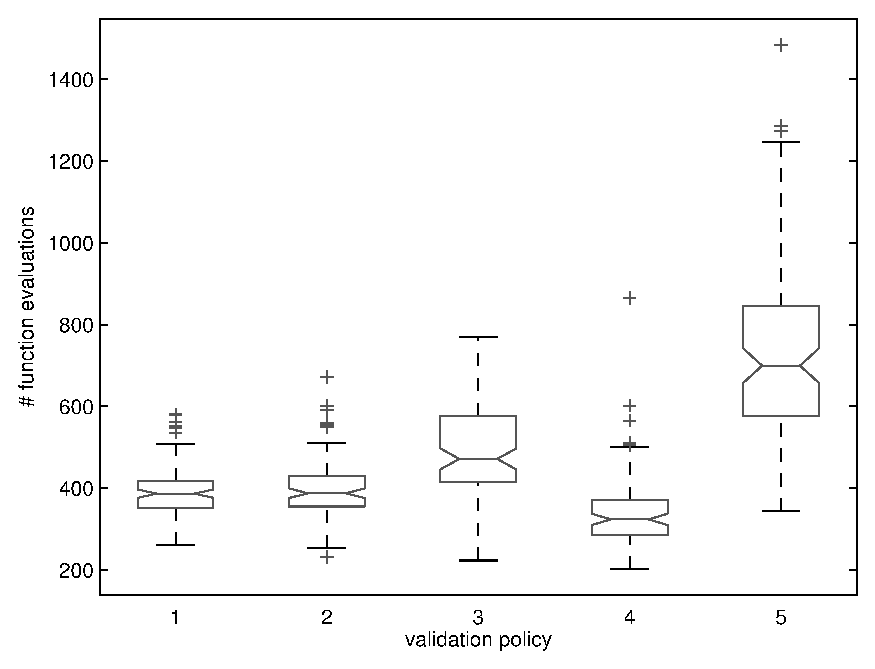
\includegraphics[width=0.80\columnwidth]{anova}
\caption{Anova plot for different validation strategies: 1) prune old individuals, 2) prune bad individuals, 3) adding a pseudo mean candidate individual 
4) correctly rank $\mu$ best ranked candidate individuals 5) update on every other generation for Rosenbrock's function for dimension $n=2$}
\label{fig:anova}
\end{figure}

The surrogate ranking validation and improvement strategy using ordinal regression is tested using a covariance matrix adaptation evolution strategy (CMA-ES) \cite{hansen:ostermeier:01}. CMA-ES is a very efficient numerical optimization technique, however we still expect to reduce the number of function evaluations needed for search. In \cite{Ru06:PPSN} the validation policy had to successfully rank all of the candidate individuals, i.e. until $\tau=1$. %<viðbót vegna rýnis>
If there is no limit to training size then updating the surrogate becomes too computationally expensive, hence the training size needs to be pruned to size to $\overline{\ell}$. %</viðbót vegna rýnis>
In \cite{Ru06:PPSN} the set was pruned to a size $\overline{\ell} = \lambda$ by omitting the oldest individuals first. These are quite stringent restrictions which can be improved upon. 
% Pruning away the worst - instead of the oldest 
The pruning only considers the age of the individuals, however older individuals might still be of more interest than newer ones if their fitness ranks higher. Thus a more sophisticated way of pruning would be omitting the lowest ranking individuals first. 
% Validating on a mean pseudo individual  
Moreover, candidate individuals are generated randomly using a normal distribution, thus a pseudo individual representing their mean could be of interest as an indicator for the entire population, e.g. by validating this pseudo individual first could give information if the surrogate is outdated w.r.t. the current search space. 
% Validation only the current mu best ranked individuals 
Furthermore, the validation is only done on the candidate individuals for the current generation in ES where only the $\mu$ best ranked individuals will survive to become parents. In evolutionary computing one is interested in the accurate ranking of individuals  generated in the neighborhood of parent individuals, hence for sufficient validation of the surrogate, only the $\mu$ best ranked individuals  should be considered and evaluated, since all other individuals  of lower rank will be disregarded in the next iteration of ES. 
% Validating on every other generation
Lastly, one should also investigate the frequency by which the model is validated, e.g. at each generation or every $K>1$ generations or even have the need for validating adapt with time.

Preliminary tests were conducted on which validation method deemed fruitful, by implementing  Rosenbrock's function of dimension $n=2$, for 1) the setup presented in \cite{Ru06:PPSN} and comparing it with the aforementioned validation improvements, which were added one at a time. Namely; 2) omitting the worst individuals  during the pruning process, instead of the oldest ones; 3) initialize the validation process by using a pseudo individual  that represents the mean of the new candidate individuals; 4) requiring that only the $\mu$ best candidate individuals are correctly ranked; and 5) validating on every other generation. 
Experimental results focusing on the number of function evaluations are shown in Fig.~\ref{fig:anova}. There is no statistical difference between omitting oldest or worst ranked individuals  from the training set, but this was expected, since both are believed to be representatives of a region of the search space which is no longer of interest. Adding the pseudo mean candidate individual didn't increase the performance edge. When the surrogate was updated on every other generation, it quickly became outdated and more than double function evaluations were needed to achieve the same rate of convergence. 
However, requiring the correct ranking for only the $\mu$ best ranked candidate individuals showed a significant performance edge. 

If the training accuracy is not 100\% then clearly $\tau < 1$. In this case additional training individuals  would be forced for evaluation. However, enforcing a completely concordant ranking, i.e. $\tau=1$, was deemed to be too strict due to the fact the search is stochastic. Thus the surrogate is said to be sufficiently accurate if $\tau>0.999$. 

Based on these preliminary tests, a pseudo code for the proposed model validation and improvement strategy is described in Fig.~\ref{fig:improvedmodel} where it is implemented at the end of each generation of CMA-ES. The algorithm essentially only evaluates the expensive true fitness function when the surrogate is believed to have diverged. During each iteration of the validation process there are two sets of individuals, $\mathcal{Y}$ and $\mathcal{X}$, which are the training individuals  which have been evaluated with the expensive model, and the candidate individuals (of unknown fitness) for the next iteration of CMA-ES, respectively. The test individuals  of interest are those who are believed to become parent individuals  in the next generation of CMA-ES, i.e. the $\mu$ best ranked candidate individuals according to the surrogate $h$. The method uses only a simple cross-validation on a single test individual, the one which the surrogate ranks the highest and has not yet been added to the training set. Creating more test individuals  would be too costly, but plausible. Once a test individual has been evaluated it is added to the training set and the surrogate $h$ is updated w.r.t. $\mathcal{Y}$, cf. Fig.~\ref{fig:schema}. This is repeated until the surrogate is said to be sufficiently accurate, which occurs if either:
\begin{itemize}
  \item Kendall's $\tau$ statistic between the ranking of the training set using the surrogate, $\bar{R}$, and its true ranking, $R$, is higher than $0.999$, or
  \item $\mu$ best ranked candidate individuals w.r.t. the current surrogate have been added to the training set.
\end{itemize}
Note that during each update of the surrogate of the ranking of the $\mu$ best candidate individuals can change. Thus it is possible to evaluate more then $\mu$ test individuals  during each validation. 

Once the validation algorithm has completed, the training set is pruned to a size $\bar{\ell}=\lambda$ by omitting the lowest ranking individuals . 

\begin{figure}[t!]
\centering \noindent 
{\footnotesize
\begin{tabbing}
\quad \quad \= 0\;\; \= \emph{Initialization}: Let $\mathcal{Y}$ denote current training set and its \\
\>   \> corresponding surrogate by $h$. Let $\mathcal{X}$ denote population \\
\>   \> of $\lambda$ individuals of unknown fitness under inspection.\\
\>1  \> {\bf for} \= $t := 1$ to $\lambda$ {\bf do} \emph{(validate a test individual )}\\ 
\>2  \>\> Estimate ranking of $\mathcal{X}$ using $h$; denoted by $\bar{R}_0$. \\
\>3  \>\> $\vec{x}_B \leftarrow \max_{\vec{x}\in\mathcal{X}\setminus\mathcal{Y}}\left\{\bar{R}_0\right\}$ (\emph{test individual}). \\
\>4  \>\> Rank $\vec{x}_B$ w.r.t. individuals  in $\mathcal{Y}$ using $h$; denoted by $\bar{R}$. \\
\>5  \>\> Evaluate $\vec{x}_B$ using true fitness function and evaluate its\\
\>   \>\> true rank among individuals  in $\mathcal{Y}$; denoted by $R$. \\ 
% In the case where no explicit fitness function can be defined, the test individual is evaluated by comparing it with selected individuals  in the training set.
\>6  \>\> $\mathcal{Y}\leftarrow\mathcal{Y}\cup\{\vec{x}_B\}$ \emph{(add to training set)}. \\
\>7  \>\> Compare the rankings  $\bar{R}$ and $R$ by computing the rank \\
\>   \>\> correlation $\tau$.\\
\>8  \>\> {\bf if} \= $\tau>0.999$ {\bf then} \\
\>9  \>\> \> break (\emph{model is sufficiently accurate}) \\
\>10 \>\> {\bf fi} \\
%This is a simple cross-validation on a single test individual. Creating more test individuals  would be too costly, but plausible.
\>11  \>\> Update the surrogate $h$ using the new training set $\mathcal{Y}$.\\
\>12  \>\> {\bf if} \= $\mu$ best individuals of $\bar{R}_0$ have been evaluated {\bf then} \\
\>13  \>\> \> break (\emph{model is sufficiently accurate}). \\
\>14  \>\> {\bf fi} \\
\>15  \> {\bf od}\\
%  Repeated the steps 1-9 above until $\tau_t>0.999$ or at least the $\mu$  highest ranking individuals  of unknown fitness have been evaluated. There is no need to evaluate more than the $\mu$ best ranking individuals  since they will be disregarded in the next iteration of CMA-ES.
\end{tabbing}}
\caption{Sampling strategy to validate and improve surrogate models.}\label{fig:improvedmodel}
\end{figure}

\begin{figure}[t!]
\centering 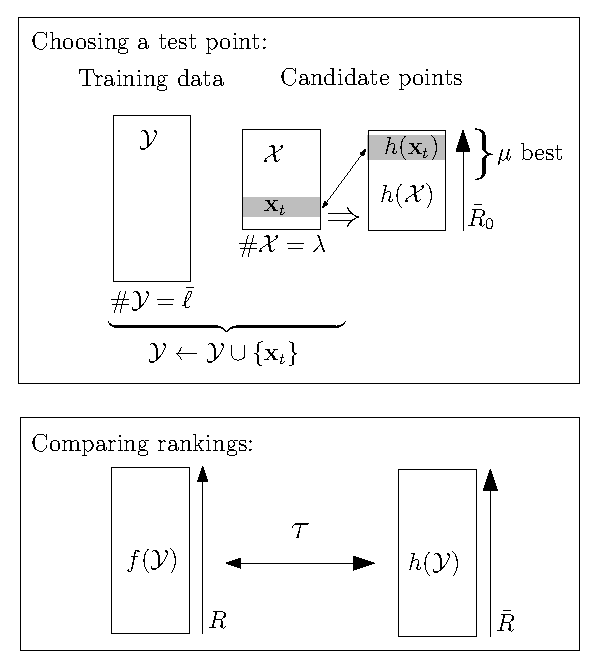
\includegraphics[width=0.6\columnwidth]{schema}
\caption{Schema for the sampling strategy.}\label{fig:schema} 
\end{figure}

\section{Experimental Study}\label{sec:Experiment}
In the experimental study CMA-ES  is run for several test functions, namely sphere model and Rosenbrock's function, of various dimensions $n=2,5,10$ and $20$. The average fitness for $100$ independent runs versus the number of function evaluations is reported using the original validation procedure presented in \cite{Ru06:PPSN} and compared with its new and improved validation procedure presented in Fig.~\ref{fig:improvedmodel}, % <viðbót vegna bls. takmarka>
the procedures will be referred to as using ``all'' or only the ``$\mu$ best'' candidate individuals during the validation, respectively. % </viðbót vegna bls. takmarka>
The parameter setting for the $(\mu,\lambda)$ CMA-ES is as recommended in \cite{hansen:ostermeier:01} with population size $\lambda = 4+\lfloor 3\ln(n)\rfloor$ and the number of parents selected $\mu=\lambda/4$. The stopping criteria used are $1000n$ function evaluation or a fitness less than $10^{-10}$. The initial mean search individual is generated from a uniform distribution between $0$ and $1$. It is also noted that the training set is only pruned to size $\overline{\ell} = \lambda$ subsequent to the validation and improvement procedure introduced in Fig.~\ref{fig:improvedmodel}. 

\subsection{Sphere model}\label{sec:sphere}
The first experimental results are presented for the unimodal sphere model of dimension $n$, 
\begin{equation} f(\vec{x}) = \sum_{i=1}^nx_i^2.\end{equation}
The average fitness versus the number of function evaluations is presented in Fig.~\ref{fig:sphereFitness}. A performance edge is achieved by restricting the validation strategy to only having the surrogate correctly rank the $\mu$ highest ranking individuals, and thereby saving the algorithm of evaluating individuals  that would have been disregarded in the next iteration. Fig.~\ref{fig:sphereIntmEval} shows the mean intermediate function evaluations that are calculated during the validation process. As one expects, requiring the method to evaluate no more than the $\mu$ best ranked candidate individuals results in a lower intermediate function evaluations, generally saving the method one function evaluation per generation, it also achieves a better mean fitness, as shown in Table~\ref{tbl:Sphere}.

\begin{figure}[b!]
\centering
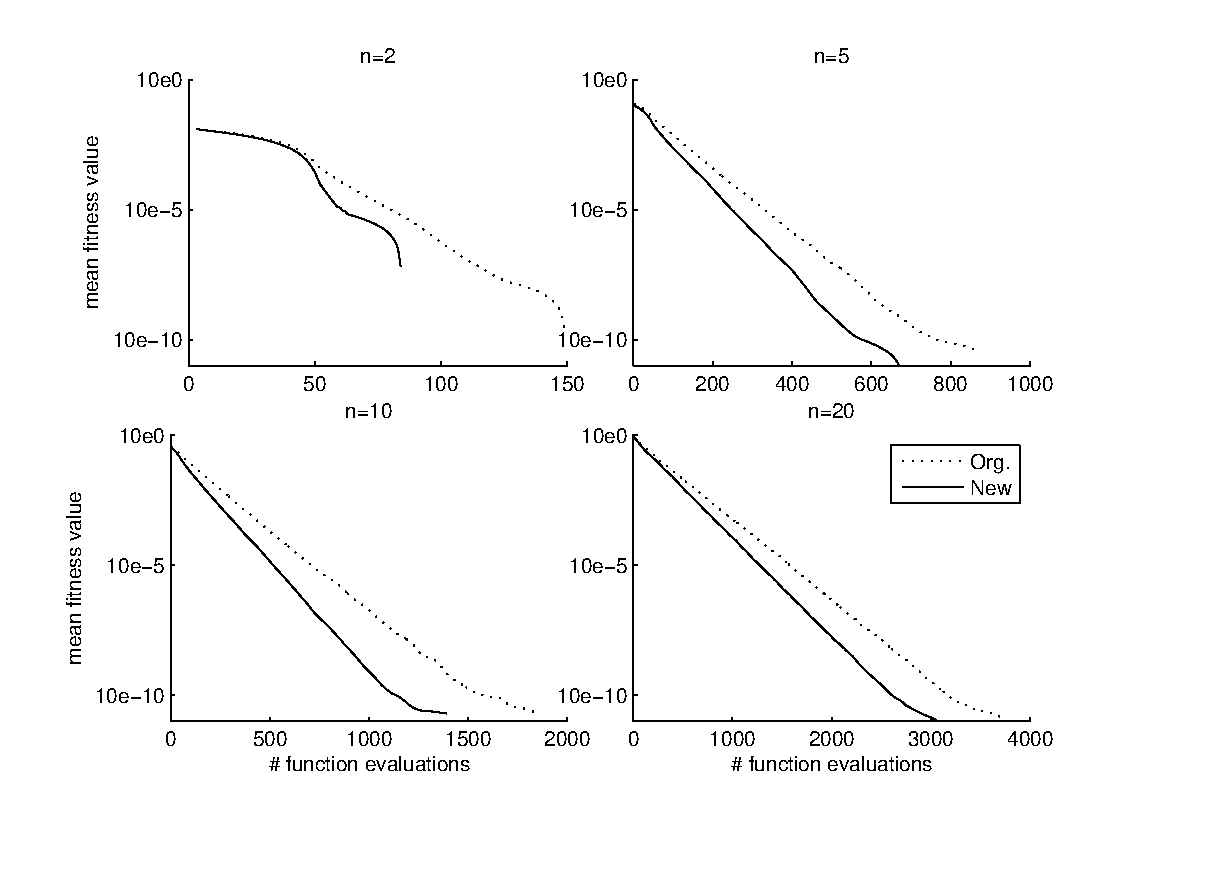
\includegraphics[trim = 8mm 10mm 10mm 5mm, clip, width=0.8\columnwidth]{sphere_meanFitness_funcEval}
\caption{Mean fitness values versus number of function evaluation by updating surrogate using all (dotted) or $\mu$ best (solid) individuals for sphere model.}
\label{fig:sphereFitness}
\end{figure}
\begin{figure}[t!]
\centering
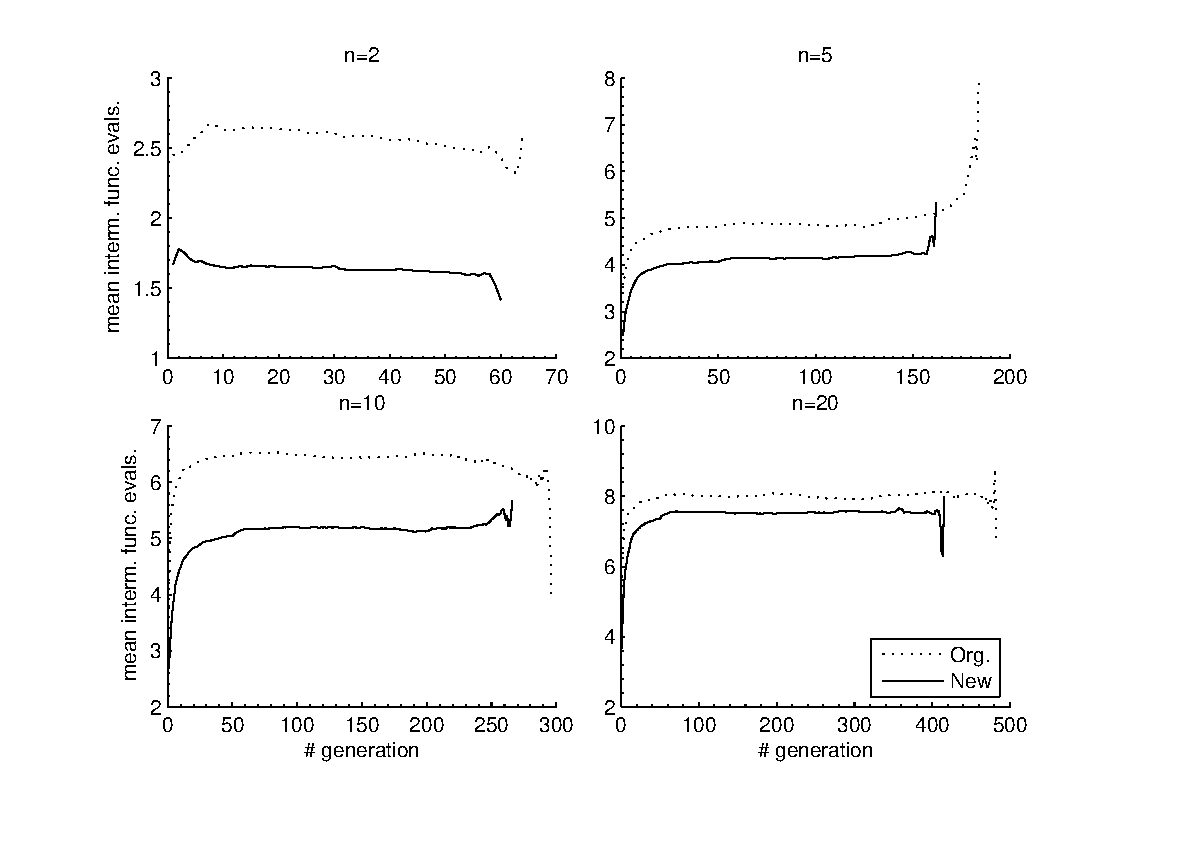
\includegraphics[trim = 10mm 10mm 10mm 5mm, clip, width=0.8\columnwidth]{sphere_intmEvals_gen}
\caption{Mean intermediate function evaluations versus generation by updating surrogate using all (dotted) or  $\mu$ best (solid) individuals for sphere model.}
\label{fig:sphereIntmEval}
\end{figure}

\begin{table}[t!] 
\centering
{\renewcommand{\arraystretch}{1.1} \renewcommand{\tabcolsep}{0.04cm} \scriptsize%footnotesize
\begin{tabularx}{0.99\columnwidth}{| X | c | rrr | rrr| rrr |}
\hline
 & & \multicolumn{3}{c|}{Function eval.} & \multicolumn{3}{c|}{Generations} & \multicolumn{3}{c|}{Fitness} \\ 
     & $n$ & \multicolumn{1}{|c}{mean} & \multicolumn{1}{c}{median} & \multicolumn{1}{c|}{sd} & \multicolumn{1}{|c}{mean} & \multicolumn{1}{c}{median} & \multicolumn{1}{c|}{sd} & \multicolumn{1}{|c}{mean} & \multicolumn{1}{c}{median} & \multicolumn{1}{c|}{sd} \\
\hline
all& 2 & 130.59 & 132 & 18.33 & 49.02 & 49 & 6.51 & 2.35e-09 & 2.82e-10 & 1.15e-08\\ 
$\mu$&2 & 81.53 & 81 & 9.53 & 48.11 & 48 & 5.02 & 7.01e-10 & 2.26e-10 & 1.35e-09\\ \hline
all& 5 & 702.02 & 702 & 67.57 & 145.15 & 145 & 14.96 & 2.77e-10 & 1.82e-10 & 3.64e-10\\ 
$\mu$& 5 & 545.25 & 547 & 54.27 & 132.60 & 132 & 11.03 & 1.83e-10 & 1.46e-10 & 1.09e-10\\ \hline
all& 10 & 1563.58 & 1553 & 117.09 & 241.83 & 240 & 18.47 & 1.52e-10 & 1.37e-10 & 5.03e-11\\ 
$\mu$& 10 & 1161.03 & 1158 & 79.98 & 226.60 & 224 & 13.86 & 1.34e-10 & 1.22e-10 & 3.80e-11\\ \hline
all& 20 & 3383.83 & 3377 & 135.52 & 423.14 & 424 & 20.42 & 1.27e-10 & 1.21e-10 & 2.51e-11\\ 
$\mu$& 20 & 2795.28 & 2804 & 132.77 & 372.86 & 372 & 16.56 & 1.17e-10 & 1.12e-10 & 1.72e-11\\ \hline
\end{tabularx}
}
\caption{Main statistics of experimental results for updating surrogate with all or $\mu$ best individuals on sphere model.}\label{tbl:Sphere}
\end{table}

\subsection{Rosenbrock's function}\label{sec:rosen}
The first experiment is now repeated for Rosenbrock's function, 
\begin{equation}f(\vec{x}) = \sum_{i=2}^n 100(x_{i}-x_{i-1}^2)^2 + (1-x_{i-1})^2.\end{equation}
The average fitness versus the number of function evaluations is presented in Fig.~\ref{fig:rosenFitness} and Fig.~\ref{fig:rosenIntmEval} shows the mean intermediate function evaluations that are calculated during the validation process. Despite requiring more generations, the over all function evaluations are significantly lower and yield a better fitness when updating the surrogate on only the $\mu$ best individuals as shown in Table~\ref{tbl:Rosenbrock}. If all of the candidate individuals have to be ranked correctly, the method will get stuck in local minima for this problem in around 6 out of 100 experiments, however this is not a problem if only the $\mu$ best candidate individuals are ranked consistently, except at high dimensions, and even then the $\mu$ best individuals  policy significantly outperforms evaluating all of the candidate individuals. Clearly the choice of validation policy will influence search performance. 
\begin{figure}[b!]
\centering
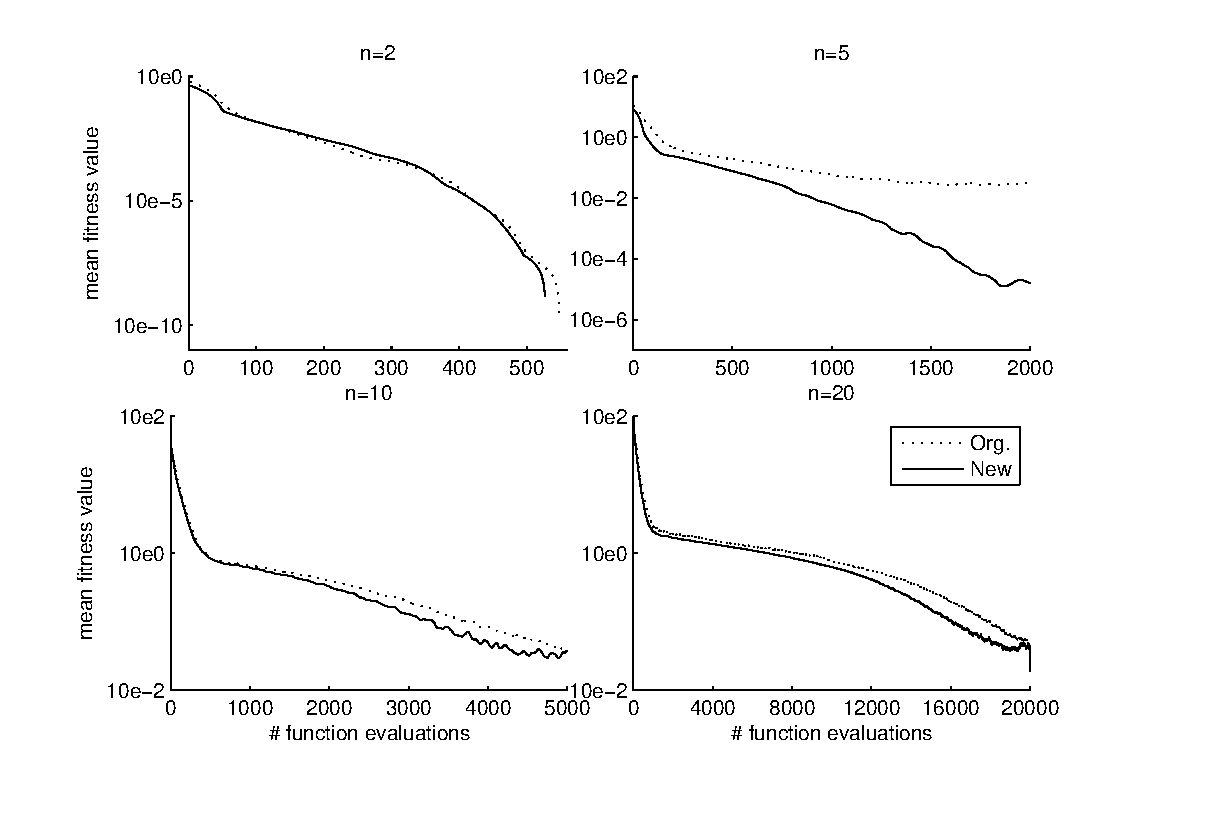
\includegraphics[trim = 10mm 10mm 10mm 5mm, clip, width=0.8\columnwidth]{rosen_meanFitness_funcEval}
\caption{Mean fitness values versus number of function evaluation by updating surrogate using all (dotted) or $\mu$ best (solid) individuals for Rosenbrock's function.}
\label{fig:rosenFitness}
\end{figure}
\begin{figure}[t!]
\centering
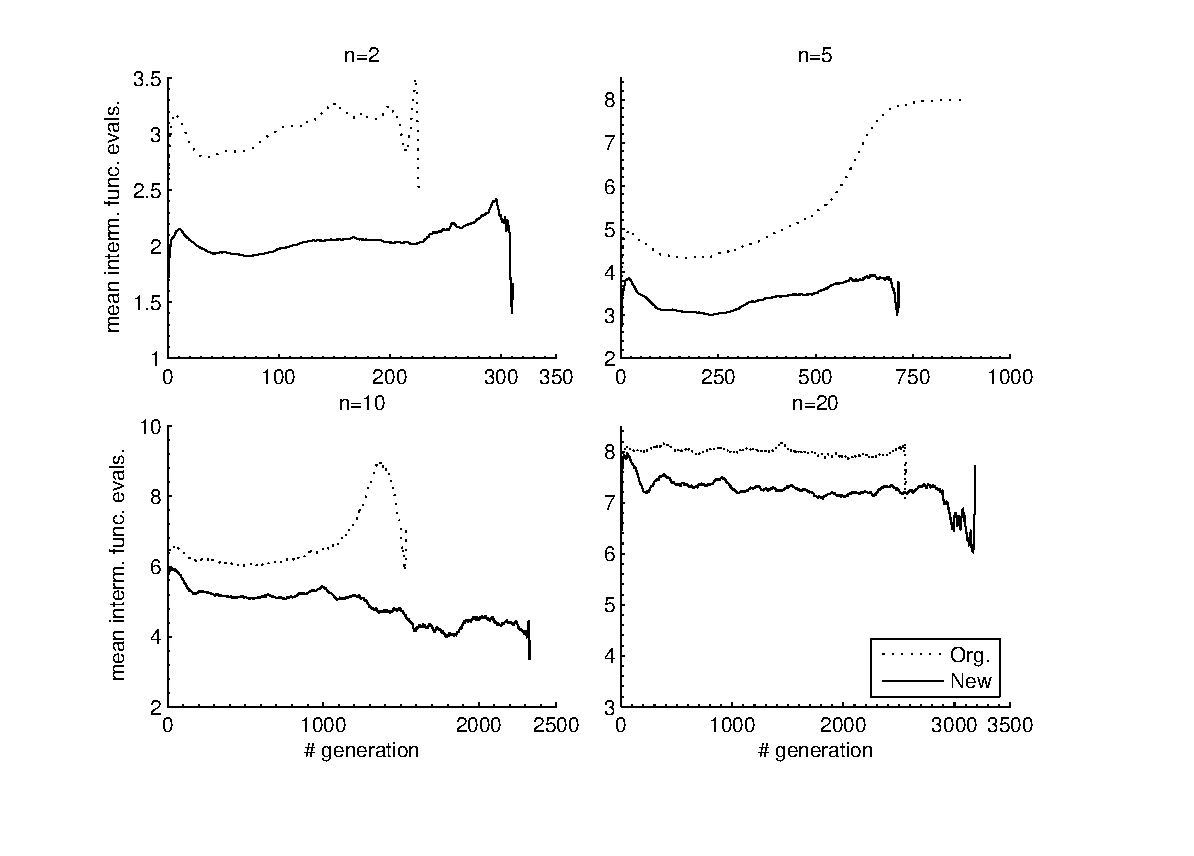
\includegraphics[trim = 15mm 10mm 15mm 5mm, clip, width=0.8\columnwidth]{rosen_intmEvals_gen}
\caption{Mean intermediate function evaluations versus generation by updating surrogate using all (dotted) or $\mu$ best (solid) individuals for Rosenbrock's function.}
\label{fig:rosenIntmEval}
\end{figure}

\begin{table}[t!]
\centering
{\renewcommand{\arraystretch}{1.1} \renewcommand{\tabcolsep}{0.02cm} \scriptsize%footnotesize
\begin{tabularx}{0.99\columnwidth}{| X | c | rrr | rrr| rrr |}
\hline
 & & \multicolumn{3}{c|}{Function eval.} & \multicolumn{3}{c|}{Generations} & \multicolumn{3}{c|}{Fitness} \\ 
     & $n$ & \multicolumn{1}{|c}{mean} & \multicolumn{1}{c}{median} & \multicolumn{1}{c|}{sd} & \multicolumn{1}{|c}{mean} & \multicolumn{1}{c}{median} & \multicolumn{1}{c|}{sd} & \multicolumn{1}{|c}{mean} & \multicolumn{1}{c}{median} & \multicolumn{1}{c|}{sd} \\
\hline
all & 2 & 389.85 & 386 & 63.85 & 132.31 & 130 & 31.25 & 6.24e-10 & 3.20e-10 & 1.05e-09\\ 
$\mu$ & 2 & 344.91 & 336 & 78.58 & 172.16 & 170 & 49.95 & 7.53e-10 & 1.66e-10 & 3.64e-09\\ \hline
all & 5 & 2464.22 & 2280 & 748.55 & 514.59 & 492 & 105.77 & 2.75e-01 & 1.74e-10 & 1.01e+00\\ 
$\mu$ & 5 & 1724.89 & 1729 & 295.60 & 520.66 & 520 & 82.79 & 1.83e-10 & 1.53e-10 & 1.05e-10\\ \hline
all & 10 & 6800.50 & 6495 & 1258.68 & 1079.82 & 1052 & 177.76 & 2.79e-01 & 1.32e-10 & 1.02e+00\\ 
$\mu$ & 10 & 6138.48 & 6143 & 1398.15 & 1177.71 & 1103 & 310.11 & 1.99e-01 & 1.24e-10 & 8.73e-01\\ \hline
all & 20 & 19968.80 & 20004 & 234.66 & 2494.00 & 2500 & 49.60 & 4.54e-01 & 2.88e-02 & 1.08e+00\\ 
$\mu$ & 20 & 19645.90 & 20002 & 1086.37 & 2687.25 & 2748 & 230.50 & 3.10e-01 & 3.12e-07 & 9.97e-01\\ \hline
\end{tabularx}
}
\caption{Main statistics of experimental results for updating surrogate with all or $\mu$ best individuals on Rosenbrock's function.} \label{tbl:Rosenbrock}
\end{table}

% An example of a floating figure using the graphicx package.
% Note that \label must occur AFTER (or within) \caption.
% For figures, \caption should occur after the \includegraphics.
% Note that IEEEtran v1.7 and later has special internal code that
% is designed to preserve the operation of \label within \caption
% even when the captionsoff option is in effect. However, because
% of issues like this, it may be the safest practice to put all your
% \label just after \caption rather than within \caption{}.
%
% Reminder: the "draftcls" or "draftclsnofoot", not "draft", class
% option should be used if it is desired that the figures are to be
% displayed while in draft mode.
%
%\begin{figure}[!t]
%\centering
%\includegraphics[width=2.5in]{myfigure}
% where an .eps filename suffix will be assumed under latex, 
% and a .pdf suffix will be assumed for pdflatex; or what has been declared
% via \DeclareGraphicsExtensions.
%\caption{Simulation Results}
%\label{fig_sim}
%\end{figure}

% Note that IEEE typically puts floats only at the top, even when this
% results in a large percentage of a column being occupied by floats.


% An example of a double column floating figure using two subfigures.
% (The subfig.sty package must be loaded for this to work.)
% The subfigure \label commands are set within each subfloat command, the
% \label for the overall figure must come after \caption.
% \hfil must be used as a separator to get equal spacing.
% The subfigure.sty package works much the same way, except \subfigure is
% used instead of \subfloat.
%
%\begin{figure*}[!t]
%\centerline{\subfloat[Case I]\includegraphics[width=2.5in]{subfigcase1}%
%\label{fig_first_case}}
%\hfil
%\subfloat[Case II]{\includegraphics[width=2.5in]{subfigcase2}%
%\label{fig_second_case}}}
%\caption{Simulation results}
%\label{fig_sim}
%\end{figure*}
%
% Note that often IEEE papers with subfigures do not employ subfigure
% captions (using the optional argument to \subfloat), but instead will
% reference/describe all of them (a), (b), etc., within the main caption.


% An example of a floating table. Note that, for IEEE style tables, the 
% \caption command should come BEFORE the table. Table text will default to
% \footnotesize as IEEE normally uses this smaller font for tables.
% The \label must come after \caption as always.
%
%\begin{table}[!t]
%% increase table row spacing, adjust to taste
%\renewcommand{\arraystretch}{1.3}
% if using array.sty, it might be a good idea to tweak the value of
% \extrarowheight as needed to properly center the text within the cells
%\caption{An Example of a Table}
%\label{table_example}
%\centering
%% Some packages, such as MDW tools, offer better commands for making tables
%% than the plain LaTeX2e tabular which is used here.
%\begin{tabular}{|c||c|}
%\hline
%One & Two\\
%\hline
%Three & Four\\
%\hline
%\end{tabular}
%\end{table}


% Note that IEEE does not put floats in the very first column - or typically
% anywhere on the first page for that matter. Also, in-text middle ("here")
% positioning is not used. Most IEEE journals/conferences use top floats
% exclusively. Note that, LaTeX2e, unlike IEEE journals/conferences, places
% footnotes above bottom floats. This can be corrected via the \fnbelowfloat
% command of the stfloats package.


\section{Discussion and Conclusion}\label{sec:Discussion}
The technique presented in this paper to control the number of true fitness evaluations is based on a single test individual chosen from a set of candidate individuals which the surrogate ranks the highest. The approximate ranking of this test individual is compared with its true ranking in order to determine the quality of the surrogate. This is a simple form of cross-validation. An alternative approach could be to rank all candidate individuals along with the training individuals  using the surrogate model. This is followed by the re-ranking of training and candidate individuals using the updated surrogate and comparing it with the previous estimate by computing Kendall's $\tau$. Its aim is to observe a change in ranking between successive updates of the surrogate. This study has shown that during the validation process it is sufficient for $\tau$ to be close to $1$ or that only the potential parent individuals  should be ranked consistently. Moreover, the new validation approach reduces the number of fitness evaluation needed, without a loss in performance although it might take a few more iterations in CMA-ES. The studies presented are exploratory in nature and clearly the approach must be evaluated on a greater range of test functions. %<viðbót vegna rýnis>
These investigations are currently underway for combinatorial optimization problem, e.g. job shop scheduling problem.  %</viðbót vegna rýnis>

When it comes to modeling surrogates based on training data, the general rule of thumb is the bigger the training set, the more accurate a model. However, there are computational time limits thus pruning of the training set is necessary. Previous studies \cite{Jin2005,Ratle1999} have reported that replacing random training individuals  is not optimal. This study has shown that there is no statistical difference in omitting oldest or lowest-ranking individuals  from the training set. Hence, for future work, further investigation on the fitness landscape is needed to determine effectively which search area is no longer of interest and thus unnecessary for the surrogate to approximate correctly. For instance it could be of interest to disregard training individuals  with the largest euclidean distance away from the current candidate individuals rather than simply omitting the oldest/lowest-ranking training individuals. 

When building surrogates in evolutionary computation one is interested in the quality of ranking of individuals  only. For this reason the training accuracy and cross validation is a more meaningful measure of quality for the surrogate model. This is in contrast to regression, where the fitness function is modeled directly and the quality estimated in terms of measures such a least square error. 
This study has shown that the sampling used for validating the accuracy of the surrogate can stop once the $\mu$ best ranked candidate individuals have been evaluated, since they are the only candidate individuals who will survive to become parents in the next generation. 
Although in some cases the sampling could stop sooner, when the surrogate ranking and true ranking are sufficiently concordant, i.e. $\tau$ was close to 1. This slight slack in for $\tau$ is allowed due to the fact the ES search is stochastic, however the allowable range in slack for $\tau$ needs to be investigated more fully % <viðbót vegna rýnis>
since allowing only $\tau\in[0.999,1]$ might be too narrow an interval, resulting in an excess of expensive function evaluations needed. %</viðbót vegna rýnis>

However, in the context of surrogate-assisted optimization the discrepancy between the exact model and its surrogate can be translated as noise, which could be an indicator of the necessary sampling size for validation/updating the surrogate, instead of only focusing on consistently ranking the $\mu$ best candidate individuals. Therefore, one can take inspiration from a varying random walk population model suggested by \cite{Miller1997} to approximate the population sizing to overcome unnecessary fitness evaluations.

% conference papers do not normally have an appendix


% use section* for acknowledgement
%\section*{Acknowledgment}
%The authors would like to thank... more thanks here


% trigger a \newpage just before the given reference
% number - used to balance the columns on the last page
% adjust value as needed - may need to be readjusted if
% the document is modified later
%\IEEEtriggeratref{8}
% The "triggered" command can be changed if desired:
%\IEEEtriggercmd{\enlargethispage{-5in}}
% references section

% can use a bibliography generated by BibTeX as a .bbl file
% BibTeX documentation can be easily obtained at:
% http://www.ctan.org/tex-archive/biblio/bibtex/contrib/doc/
% The IEEEtran BibTeX style support page is at:
% http://www.michaelshell.org/tex/ieeetran/bibtex/
\bibliographystyle{IEEEtran}
% % argument is your BibTeX string definitions and bibliography database(s)
\bibliography{isda2011}
%
% <OR> manually copy in the resultant .bbl file
% set second argument of \begin to the number of references
% (used to reserve space for the reference number labels box)


% that's all folks
\end{document}


